\section{坐标系}

这些宏替代了 \tkzname{tkz-base} 中的对应宏（\tkzcname{tkzInit}、\tkzcname{tkzGrid}、\tkzcname{tkzAxeXY}、\tkzcname{tkzDrawX}、\tkzcname{tkzClip}、\tkzcname{tkzRep}、\tkzcname{tkzText}）。

\subsection{初始化：\tkzcname{tkzFnInit}}

\begin{NewMacroBox}{tkzFnInit}{\oarg{options}}
\begin{tabular}{lll}
\toprule
选项             & 默认值 & 说明  \\
\midrule
\TOline{xmin}{-5}{最小 $x$ 值}
\TOline{xmax}{5}{最大 $x$ 值}
\TOline{xstep}{1}{$x$ 轴上 1 厘米代表的值}
\TOline{ymin}{-5}{最小 $y$ 值}
\TOline{ymax}{5}{最大 $y$ 值}
\TOline{ystep}{1}{$y$ 轴上 1 厘米代表的值}
\TOline{xorigin}{0}{$x$ 轴原点放置在 $X=0$ 处（例如某一年）}
\TOline{yorigin}{0}{$y$ 轴原点放置在 $Y=0$ 处}
\TOline{enlarge}{0（无值时为 0.1）}{按窗口尺寸的比例放大窗口}
\TOline{enlarge x, enlarge y}{enlarge}{仅在一个方向上放大}
\bottomrule
\end{tabular}

\emph{参数值可以是表达式：\texttt{xmax=2*pi}。}
\end{NewMacroBox}

\subsection{网格：\tkzcname{tkzFnGrid}}

\begin{NewMacroBox}{tkzFnGrid}{\oarg{options}\parg{$x_1$,$y_1$}\parg{$x_2$,$y_2$}}
\emph{区域参数可选；默认情况下网格覆盖整个窗口。}

\begin{tabular}{lll}
\toprule
选项             & 默认值 & 说明  \\
\midrule
\TOline{dx}{xstep}{两条竖线之间的距离}
\TOline{dy}{ystep}{两条横线之间的距离}
\TOline{sub}{false}{添加子网格}
\TOline{subdx}{dx/5}{子网格间距}
\TOline{subdy}{dy/5}{子网格间距}
\bottomrule
\end{tabular}

\emph{其他选项为 \TIKZ\ 选项；样式为 \tkzname{tkzfn grid}。}
\end{NewMacroBox}

\begin{tkzexample}[latex=8cm]
\begin{tikzpicture}[scale=1.25]
 \tkzFnInit[xmin=-2,xmax=3,
            ymin=-1,ymax=2]
 \tkzFnGrid[sub,color=orange]
 \tkzFnAxes
\end{tikzpicture}
\end{tkzexample}

\subsection{坐标轴：\tkzcname{tkzFnAxes}、\tkzcname{tkzFnAxisX}、\tkzcname{tkzFnAxisY}}

\begin{NewMacroBox}{tkzFnAxes}{\oarg{options}}
\emph{绘制两条坐标轴、刻度及其标签。若原点 $(0, 0)$ 在窗口内，则坐标轴在该点相交；否则在 $(x_{\min}, y_{\min})$ 处相交。数值按美式或法式格式书写（见第~\ref{sec:format} 节）。}

\begin{tabular}{lll}
\toprule
选项             & 默认值 & 说明  \\
\midrule
\TOline{dx, dy}{xstep, ystep}{两个刻度之间的距离}
\TOline{xlabel, ylabel}{\$x\$, \$y\$}{坐标轴名称}
\TOline{ticks}{true}{刻度线}
\TOline{labels}{true}{刻度标签}
\TOline{line}{true}{坐标轴线}
\TOline{origin}{0 或 O}{原点标签（美式为 0，法式为 O）}
\TOline{trig}{0}{若 $n>0$，$x$ 轴刻度标注为 $\pi/n$ 的倍数}
\TOline{decimals}{4}{最大小数位数}
\TOline{arrows}{end}{箭头：\texttt{end}、\texttt{both} 或 \texttt{none}（见第~\ref{sec:arrows} 节）}
\TOline{box}{false}{"矩形框"坐标轴（见第~\ref{sec:box} 节）}
\TOline{style}{school}{\texttt{school} 或 \texttt{box}}
\TOline{tick length}{3pt}{刻度线长度（矩形框模式）}
\bottomrule
\end{tabular}

\emph{\tkzcname{tkzFnAxisX} 和 \tkzcname{tkzFnAxisY} 仅绘制单条坐标轴；它们的选项相同，但使用 \tkzname{label}、\tkzname{label style} 和 \tkzname{step} 代替 \tkzname{xlabel}、\tkzname{ylabel} 和 \tkzname{dx}。设置 \tkzname{ticks=false} 时，效果等同于 \tkzcname{tkzDrawX}。}
\end{NewMacroBox}

\begin{tkzexample}[latex=8cm]
\begin{tikzpicture}
  \tkzFnInit[xmin=-7,xmax=7,
             ymin=-1,ymax=1]
  \tkzFnAxisY
  \tkzFnAxisX[trig=2]
  \tkzFnDraw[red]{sin(x)}
\end{tikzpicture}
\end{tkzexample}

\subsection{裁剪：\tkzcname{tkzFnClip}}

\begin{NewMacroBox}{tkzFnClip}{\oarg{边距（单位 pt）}}
\emph{将后续绘图限制在窗口范围内（可按边距放大）。与 \tkzcname{clip} 类似，建议在 \tkzname{scope} 环境内使用。曲线和切线默认会被裁剪到窗口内（选项 \tkzname{clip}）。}
\end{NewMacroBox}

\subsection{单位向量：\tkzcname{tkzFnRep}}

\begin{NewMacroBox}{tkzFnRep}{\oarg{\TIKZ\ 选项}}
\emph{绘制向量 $\vec{\imath}$ 和 $\vec{\jmath}$；样式为 \tkzname{tkzfn rep}。}
\end{NewMacroBox}

\subsection{文字：\tkzcname{tkzFnText}}

\begin{NewMacroBox}{tkzFnText}{\oarg{\TIKZ\ 选项}\parg{$x$,$y$}\marg{文字}}
\emph{在坐标系中坐标为 $(x, y)$ 的点处放置文字。也可以给定点的名称：\tkzcname{tkzFnText}\texttt{[above](A)\{文字\}}。}
\end{NewMacroBox}

\begin{tkzexample}[latex=8cm]
\begin{tikzpicture}[scale=1.5]
 \tkzFnInit[xmin=-3,xmax=3,
            ymin=-1,ymax=4]
 \tkzFnGrid[sub,subdx=.5,subdy=.5]
 \tkzFnAxes
 \tkzFnDraw[domain=-3:2]{(2-x)*exp(x)}
 \tkzFnText(-2,1.25){$\mathcal{C}_{f}$}
 \tkzFnRep
\end{tikzpicture}
\end{tkzexample}

\subsection{两端箭头：\tkzname{arrows}}\label{sec:arrows}

在美国，教材和图形计算器通常在坐标轴两端各画一个箭头。\tkzcname{tkzFnAxes}、\tkzcname{tkzFnAxisX} 和 \tkzcname{tkzFnAxisY} 的 \tkzname{arrows} 选项用于选择箭头样式：
\begin{itemize}
  \item \texttt{end}（默认）：正方向一端有一个箭头；
  \item \texttt{both}：两端各有一个箭头；
  \item \texttt{none}：无箭头。
\end{itemize}
|\tkzFnSetup{arrows=both}| 可为后续所有坐标系设置箭头样式。箭头尖端形状由样式 \tkzname{tkzfn axis} 控制。

\begin{tkzexample}[latex=7cm]
\begin{tikzpicture}[scale=.6]
  \tkzFnInit[xmin=-5,xmax=5,
             ymin=-4,ymax=6]
  \tkzFnGrid
  \tkzFnAxes[arrows=both]
  \tkzFnDraw[blue,thick,<->,>=stealth,
             clip=false,domain=-4.2:4.2]{x^2/2-3}
\end{tikzpicture}
\end{tkzexample}

整篇文档使用其他箭头尖端样式：

\begin{tkzexample}[latex=7cm]
\tkzFnSetup{arrows=both}
\tikzset{tkzfn axis/.style={>=latex}}
\begin{tikzpicture}[scale=.7]
  \tkzFnInit[xmin=-2,xmax=3,xstep=.5,
             ymin=-1.5,ymax=1.5,ystep=.5]
  \tkzFnGrid[sub]
  \tkzFnAxes[dx=1]
  \tkzFnDraw[red,thick]{x^3/3-x}
\end{tikzpicture}
\tkzFnSetup{arrows=end}
\tikzset{tkzfn axis/.style={->,>=stealth}}
\end{tkzexample}

无箭头：

\begin{tkzexample}[latex=7cm]
\begin{tikzpicture}[scale=.6]
  \tkzFnInit[xmin=-1,xmax=5,
             ymin=-1,ymax=3]
  \tkzFnAxes[arrows=none]
  \tkzFnDraw{sqrt(x)}
\end{tikzpicture}
\end{tkzexample}

\newpage
\subsection{"矩形框"坐标轴：\tkzname{box}}\label{sec:box}

这种表示方式常见于科学出版物和 \tkzname{pgfplots}，在中学教材中较少见。使用 \tkzname{pgfplots} 时通过 \tkzname{axis} 环境实现；使用 \tkzname{tkz-fn} 时只需一个选项：

\begin{itemize}
  \item |\tkzFnAxes[box]|：窗口四周有边框，刻度线朝内标注在四条边上，所有数值（包括边缘处）标注在框外，无箭头也无原点标签；
  \item 坐标轴名称仅在给出时标注：|xlabel| 在框下方，|ylabel| 在左侧垂直排列；
  \item |\tkzFnSetup{axes=box}| 为后续所有坐标系设置此样式；|\tkzFnSetup{axes=school}| 恢复常规样式；
  \item \tkzcname{tkzFnDraw} 的 \tkzname{mark} 选项在每个计算点处放置标记（\tkzname{samples} 设置点数）；
  \item \tkzcname{tkzFnInit} 的 \tkzname{enlarge} 选项使曲线远离边框；默认定义域仍为 $[x_{\min}, x_{\max}]$。
\end{itemize}

边框样式为 \tkzname{tkzfn box}。以下示例复现了用 \tkzname{pgfplots} 绘制的图形。

\begin{tkzexample}[latex=7cm]
\tkzFnDef{f}{1/((1e9*x/11.778)*3.273e-8
              -3.273e-8+1)}
\begin{tikzpicture}[scale=.9]
  \tkzFnInit[xmin=0,xmax=6,
             ymin=0,ymax=1,ystep=.2]
  \tkzFnAxes[box]
  \tkzFnDraw[blue,mark=*,mark size=1.5pt,
             samples=13,domain=0:5](f)
  \tkzFnDrawData[red,mark=square*,
                 mark size=1.5pt]{.125/.744}
\end{tikzpicture}
\end{tkzexample}

默认定义域为 $[x_{\min}, x_{\max}]$：

\begin{tkzexample}[latex=7cm]
\begin{tikzpicture}[scale=.9]
  \tkzFnInit[xmin=0,xmax=6,
             ymin=0,ymax=1,ystep=.2]
  \tkzFnAxes[box]
  \tkzFnDraw[blue,mark=*,mark size=1.5pt,
             samples=25](f)
  \tkzFnDrawData[red,mark=square*,
                 mark size=1.5pt]{.125/.744}
\end{tikzpicture}
\end{tkzexample}

使用 \tkzname{enlarge}（默认 10\,\%）并标注坐标轴名称：

\begin{tkzexample}[latex=7cm]
\begin{tikzpicture}[scale=.9]
  \tkzFnInit[xmin=0,xmax=6,ymin=0,ymax=1,
             ystep=.2,enlarge]
  \tkzFnAxes[box,xlabel=$x$,
             ylabel=$f(x)$]
  \tkzFnDraw[blue,mark=*,mark size=1.5pt,
             samples=25](f)
  \tkzFnDrawData[red,mark=square*,
                 mark size=1.5pt]{.125/.744}
\end{tikzpicture}
\end{tkzexample}

\newpage
使用 |\tkzFnSetup{axes=box}| 时，网格和 $\pi$ 倍数刻度照常使用；\tkzname{smooth} 选项传递给 \TIKZ。

\begin{tkzexample}[vbox]
\tkzFnSetup{axes=box}
\begin{tikzpicture}[scale=.6]
  \tkzFnInit[xmin=-3,xmax=3,ymin=0,ymax=20000,ystep=4000]
  \tkzFnGrid
  \tkzFnAxes[xlabel=$t$,ylabel=人口]
  \tkzFnDraw[red,thick,smooth,samples=7]{2000*x^2}
\end{tikzpicture}\qquad
\begin{tikzpicture}[scale=.6]
  \tkzFnInit[xmin=-7,xmax=7,ymin=-1,ymax=1,ystep=.5]
  \tkzFnAxes[trig=2]
  \tkzFnDraw{sin(x)}
\end{tikzpicture}
\tkzFnSetup{axes=school}
\end{tkzexample}

\endinput
